{\large FSM: Linea de Pase}
\begin{center}
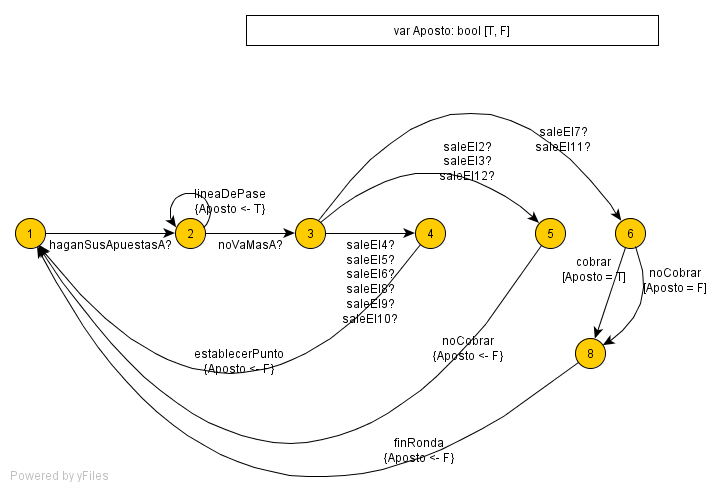
\includegraphics[scale=0.75]{img/linesDePase.png}
\end{center}

Las apuestas L�nea de Pase se efect�an antes del Tiro de Salida (\textit{haganSusApuestasA} y \textit{noVaMasA}). Si se sale un Natural (7 u 11), el Jugador cobra unicamente si aposto y la ronda termina. Si por el contrario sale un Craps (2, 3 � 12) entonces no cobra. Cualquier otro n�mero (4, 5, 6, 7, 8, 9, o 10) establece el Punto. La ronda continua hasta que se repita el Punto antes de sacar un 7 o hasta que salga un 7 antes de la repetici�n del Punto. En el primer caso cobrara si aposto y en el segundo no cobrara dado que perdio. 


\newpage

{\large FSM: Barra No Pase}
\begin{center}
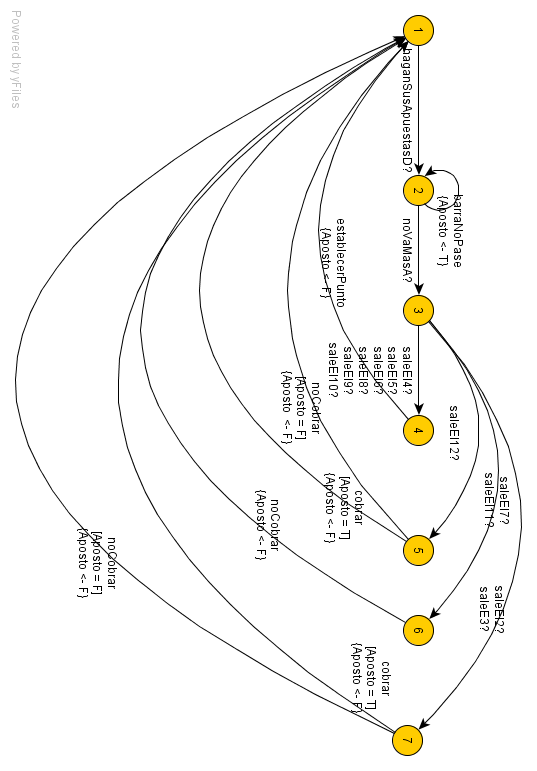
\includegraphics[scale=0.75]{img/barraNoPase.png}
\end{center}

La Barra No Pase es la apuesta contraria a la L�nea de Pase, o sea, que esta apuesta paga  solamente si el tirador lanza un 7 antes de alcanzar el Punto (si el jugador aposto), y no paga cuando el Punto es alcanzado antes de un 7. En el Tiro de Salida, la apuesta gana con un 2 o un 3, pierde con 7 u 11 y empata con un 12 (empatar significa que se devuelve el valor de la apuesta, osea que paga si se aposto o no paga de lo contrario), pues cualquier otro n�mero (4, 5, 6, 8, 9, 10) establece el Punto. 


\newpage

{\large FSM: Apuesta Venir }
\begin{center}
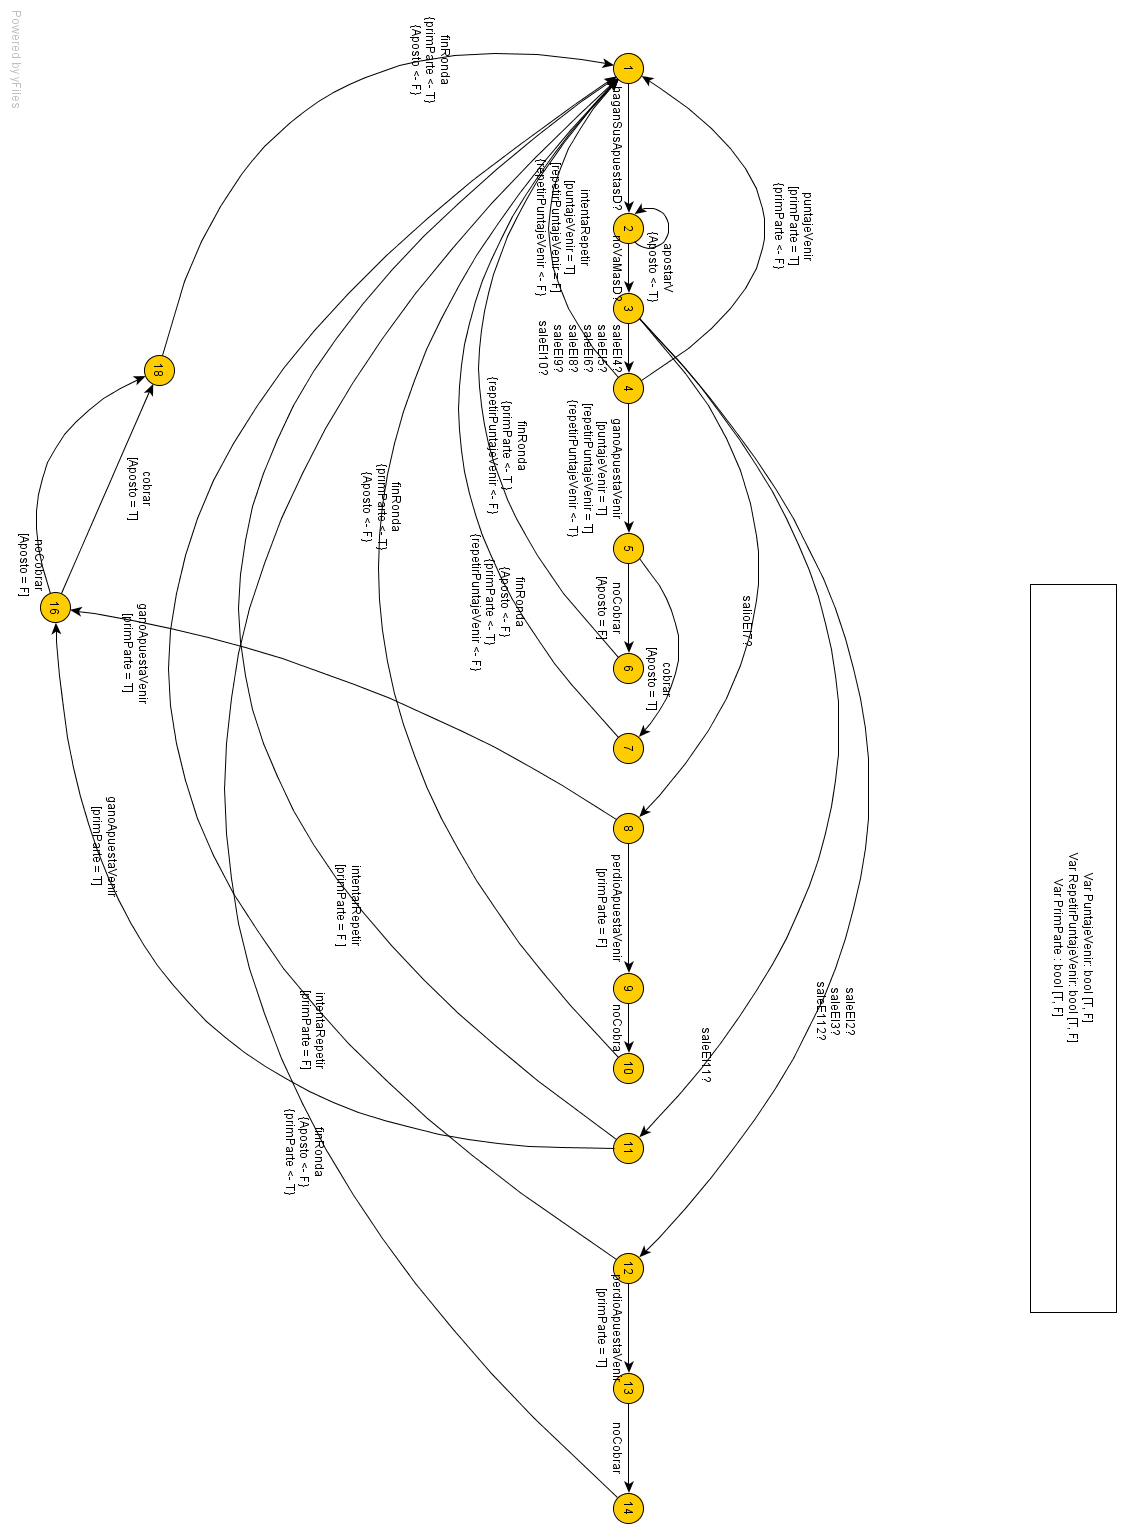
\includegraphics[scale=0.4]{img/ApuestaVenir.png}
\end{center}

Estas apuestas est�n disponibles una vez que se haya establecido el Punto y no antes (\textsl{haganSusApustasD} y \textit{noVaMasD}). Es pr�cticamente id�ntica a la propia apuesta de pase s�lo que esta se puede hacer en el medio de una ronda. El Jugador gana si en el siguiente lanzamiento de dados sale un 7 u 11, perdiendo si ese lanzamiento obtiene Craps (2, 3, o 12). Si el tirador saca 4, 5, 6, 8, 9, � 10, entonces ese n�mero se convierte en Puntaje Venir. Si el lanzador tira un Puntaje Venir nuevamente antes de obtener un 7, el Jugador gana la apuesta. Si sale un 7 primero, pierde. Si el jugador aposto y gano entonces cobrara, de lo contrario perdera su apuesta. 
Las apuestas no resueltas no pueden ser modificadas ni retiradas, y es por esta raz�n que una Apuesta Venir puede permanecer en la mesa m�s all� de la conclusi�n de la ronda. 


\newpage

{\large FSM: Apuesta No Venir}
\begin{center}
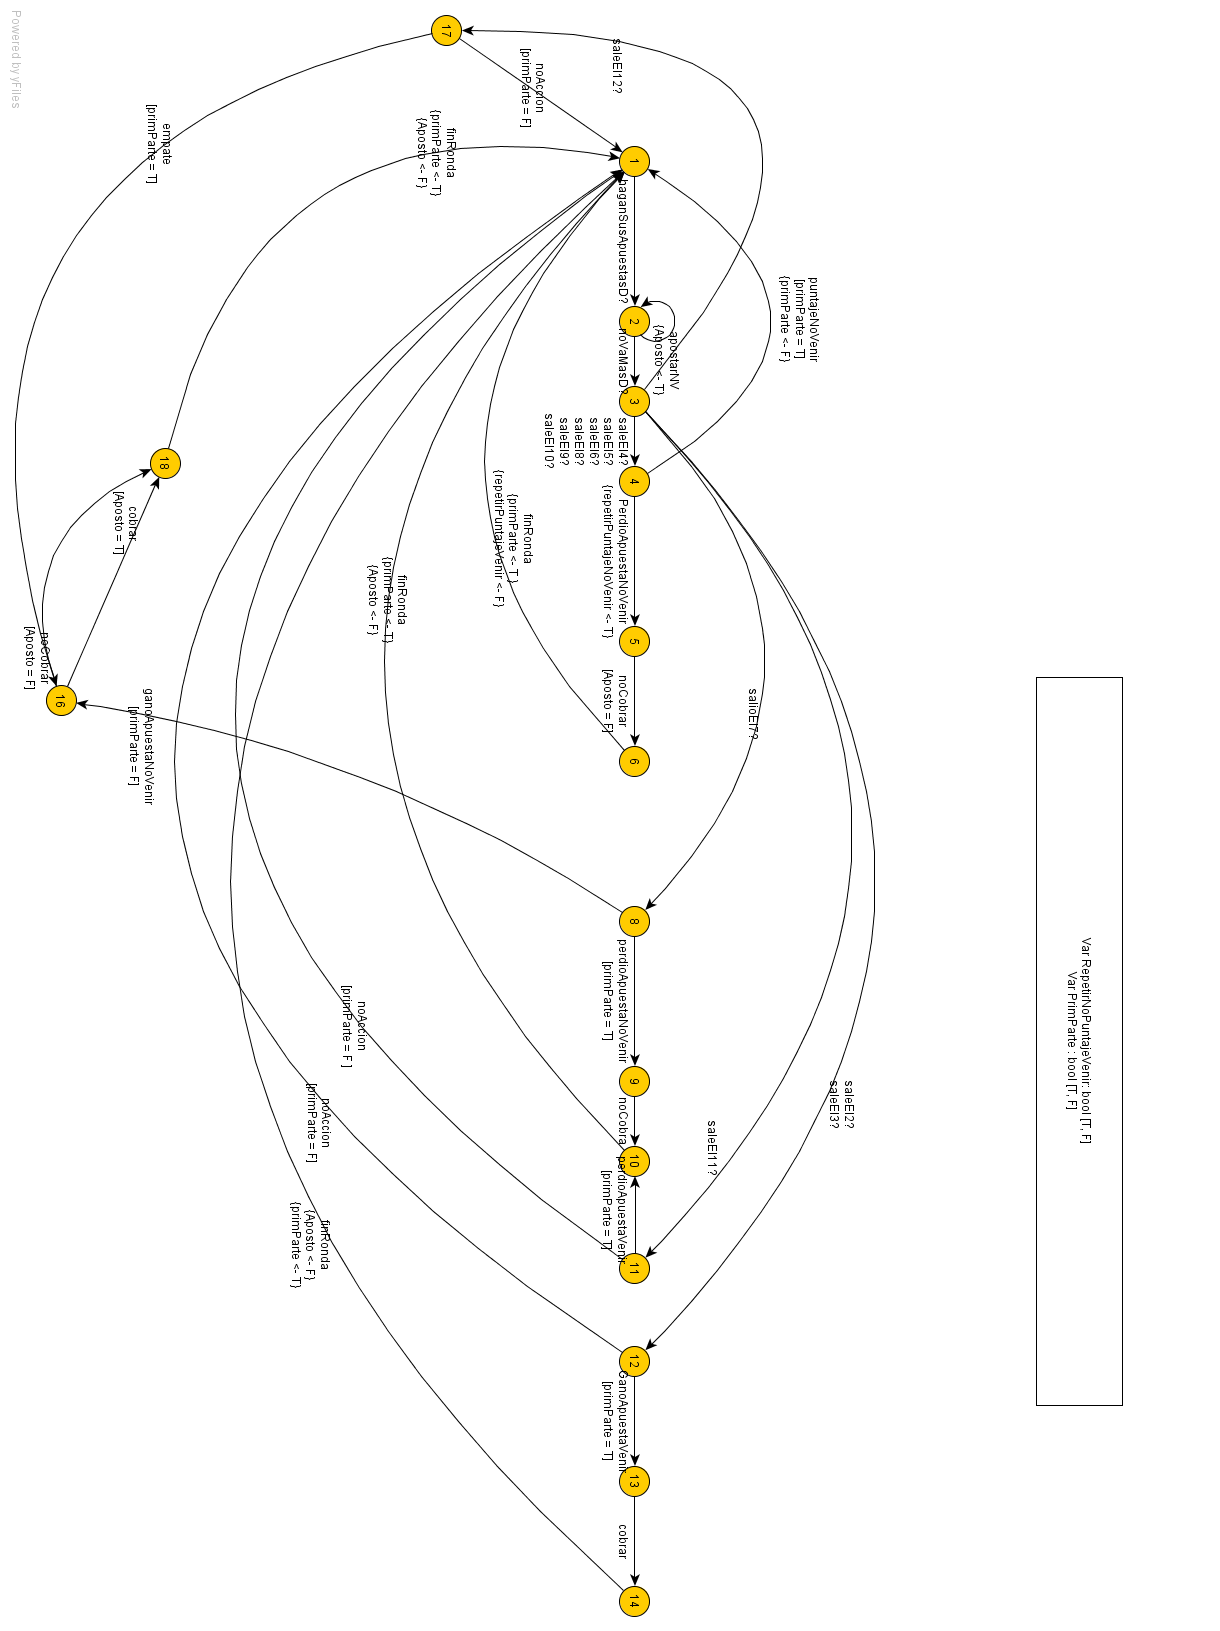
\includegraphics[scale=0.35]{img/apuestaNoVenir.png}
\end{center}

Estas apuestas est�n disponibles una vez que se haya establecido el Punto y no antes. Estas apuestas son opuestas a las Apuestas Venir. El Jugador gana si en el siguiente lanzamiento de dados sale un 2 � un 3, pierde si en ese lanzamiento salen 7 u 11, y empata (se devuelve la apuesta, de corresponder) si el lanzador tira un 12. Si el tirador saca 4, 5, 6, 8, 9, � 10, entonces ese n�mero se convierte en Puntaje No Venir. Si el lanzador tira un 7, el Jugador gana la apuesta, mientras que si saca un Puntaje No Venir, pierde. Si el jugador aposto y gano entonces cobrara, de lo contrario perdera su apuesta. 
Asi como en la \textbf{Apuesta Venir}, las apuestas no resueltas no pueden ser modificadas ni retiradas, y es por esta raz�n que una Apuesta No Venir puede permanecer en la mesa m�s all� de la conclusi�n de la ronda.

\newpage

{\large FSM: Apuesta De Campo}
\begin{center}
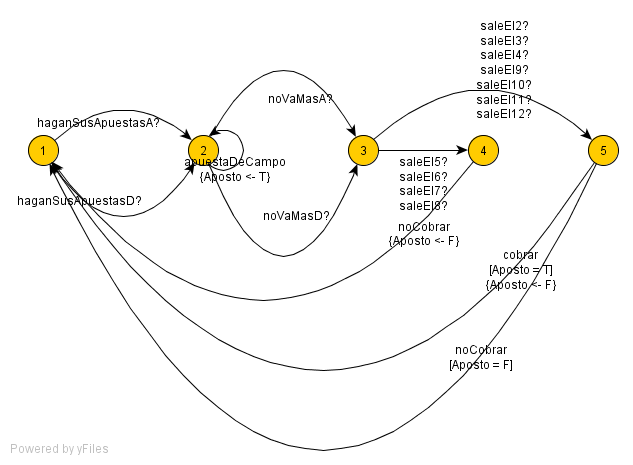
\includegraphics[scale=0.75]{img/apuestaDeCampo.png}
\end{center}

Las Apuestas de Campo son un tipo de apuesta que ganan si el lanzador saca uno de los n�meros de dicha casilla (2, 3, 4, 9, 10, 11 � 12), y pierden si saca cualquier otro valor (5, 6, 7 u 8).  Las apuestas de Campo se pueden hacer antes de cualquier tiro. 
Si el jugador aposto y gan� la apuesta entonces cobrara.

\newpage

{\large FSM: Apuesta En Sitio}
\begin{center}
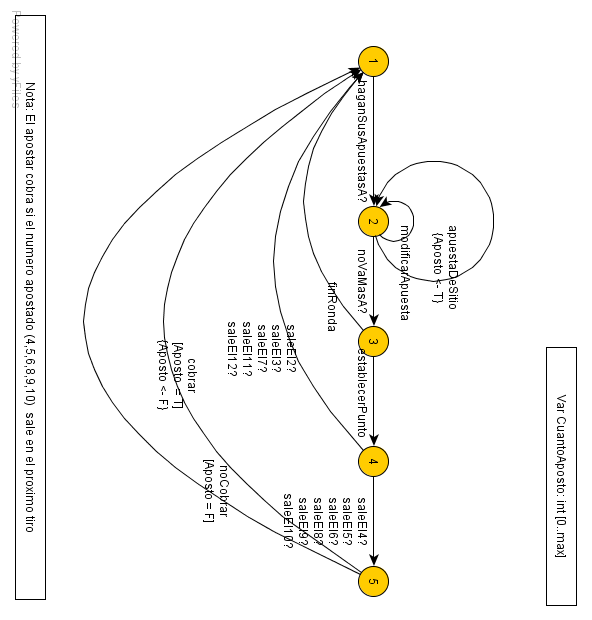
\includegraphics[scale=0.75]{img/apuestaEnSitio.png}
\end{center}


Las Apuestas en Sitio permiten apostar por o contra un n�mero de Punto espec�fico. El apostador cobrara si el numero apostado (4,5,6,8,9,10) sale en el proximo. Cobrara si hizo una apuesta.

\newpage

{\large FSM: Apuesta a Ganar}
\begin{center}
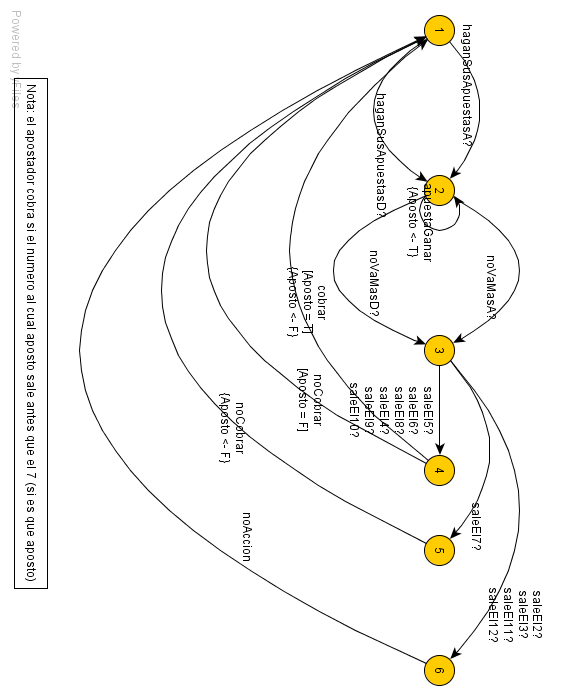
\includegraphics[scale=0.75]{img/apuestaAGanar.png}
\end{center}

Esta jugada apuesta a que saldr� un n�mero espec�fico (4, 5, 6, 8, 9, o 10) antes de que un 7 sea lanzado. Si el n�mero sale antes del 7 se gana (se cobrara si se aposto), mientras que si sale el 7 primero, se pierde (no se cobra). 
El apostador cobra si el n�mero al cual aposto sale antes que el 7 (si es que aposto).


\newpage

{\large FSM: Apuesta En Contra}
\begin{center}
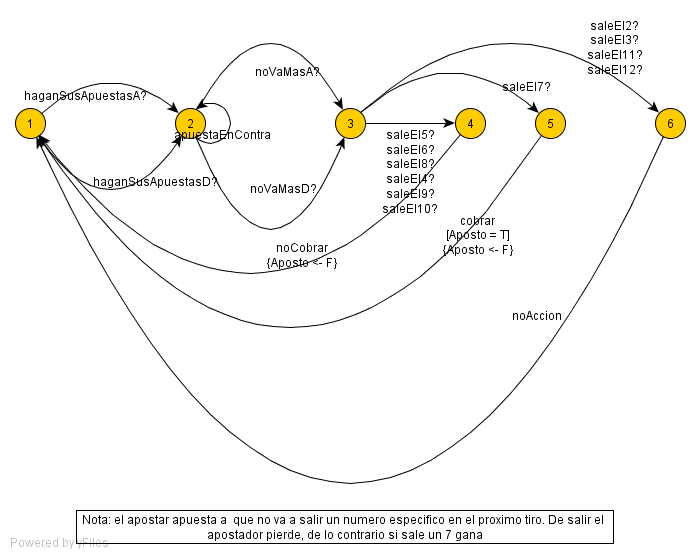
\includegraphics[scale=0.5]{img/apuestaEnContra.png}
\end{center}

Esta jugada apuesta a que saldr� un 7 antes que un n�mero espec�fico (4, 5, 6, 8, 9, o 10) sea lanzado. Si el 7 sale antes que el n�mero apostado se gana, mientras que si sale el n�mero primero, se pierde.
En este tipo de apuesta, el jugadro apuesta a que no va a salir un numero especifico en el proximo tiro. De salir el apostador pierde, de lo contrario si sale el un 7 gana y cobra si el jugador realiz� una apuesta

%\end{framed}